\chapter{Науково-методологічні основи автоматизації голосової взаємодії} \label{chapt2}

\section{Концепція створення системи голосової взаємодії} \label{sect2_1}

У результаті аналізу виявлено два найбільш перспективні напрями, поєднання яких дає змогу запропонувати нове принципове рішення і побудувати рефлекторну модель голосової взаємодії в задачах управління дистрибуцією. В основу моделі покладено логічні сценарії взаємодії на тему управління дистрибуцією, які мають враховувати параметри основних причин невідповідності реальної ситуації запланованому маршруту, наприклад, запізнення або відмови обслуговування на точці доставки тощо. Це дає змогу отримати інформацію для прийняття рішення про повернення вантажу на склад, про відміну чи відкладення обслуговування однієї точки доставки, щоб мати можливість встигнути на іншу, більш важливу, про зміну маршруту для об’їзду затору або про утворення нового маршруту з резервною машиною тощо.

Звичайно, абсолютно всі причини та параметри не можуть бути враховані заздалегідь, але проробка і врахування основної типології дозволить приймати базові рішення та вдаватися до безпосереднього зв`язку з диспетчером лише у складних випадках, що розвантажить водія та канали комунікації і дасть змогу підвищити загальну ефективність дистрибуції.

Найбільш ефективним шляхом проробки дерева сценаріїв рефлекторної взаємодії є використання вхідних параметрів вже створеної системи автоматизації дистрибуції, у тому числі автоматичної побудови маршрутів \cite{as6}, яка зараз проходить широку експериментальну апробацію. Інтеграція модулю голосової взаємодії з цією системою буде значно спрощена, що сприятиме отриманню кращого економічного ефекту.

Виходячи з наявної логіки побудови маршрутів, вже зараз можна назвати принципові блоки сценаріїв, які потрібно буде розробити. Першим етапом, на якому можуть виникнути проблеми розбіжності плану та факту, є етап завантаження на складі (якщо, наприклад, буде виявлений неврахований «перегруз» або «недогруз» машини, будуть відсутні необхідні товари чи працівники складу не встигнуть їх вчасно відібрати, або навіть виявиться, що машина не здатна вийти на маршрут (наприклад, не заводитися на морозі)).

Другий етап сценаріїв голосової взаємодії визначають проблеми, які можуть виникнути в дорозі до певної точки доставки, як, наприклад, ремонт в дорозі по маршруту руху або зміни в правилах руху на деяких вулицях, які ще не відбиті в алгоритмах прокладення маршруту (нові заборони поворотів чи односторонній рух), проблеми з автомобілем на дорозі, які призводять до зниження швидкості або відмови в подальшому русі по маршруту, або найбільш розповсюджена проблема заторів на дорогах. 

Третій етап сценаріїв голосової взаємодії викликаний можливими невідповідностями між планом та фактом в обслуговуванні на точці доставки. Це можуть бути як проблеми зі сторони клієнта («нікого немає дома», клієнт не має грошей, клієнт відмовляється від замовлення чи стверджує, що він замовляв щось інше), так і проблеми зі сторони водія (запізнення на точку доставки, тобто не потрапляння в заплановане дозволене часове вікно доступності, пошкодження товару тощо). Найбільш поширеною є ситуація, коли водій проводить в точці доставки більше часу, ніж заплановано, що призводить до проблем на всьому подальшому маршруті.

Ці та інші інциденти на всіх зазначених етапах, що зазначені в моделі на схемі (рис. \ref{img:voice_interaction_schema}), потребують вирішення із залученням диспетчера для вибору найкращої стратегії і мінімізації втрат через проблему. Відповідно дерево сценаріїв голосової взаємодії повинно відбивати всі три етапи та типові відомі проблеми і способи їх розв’язання.

\begin{figure}
	\centering
	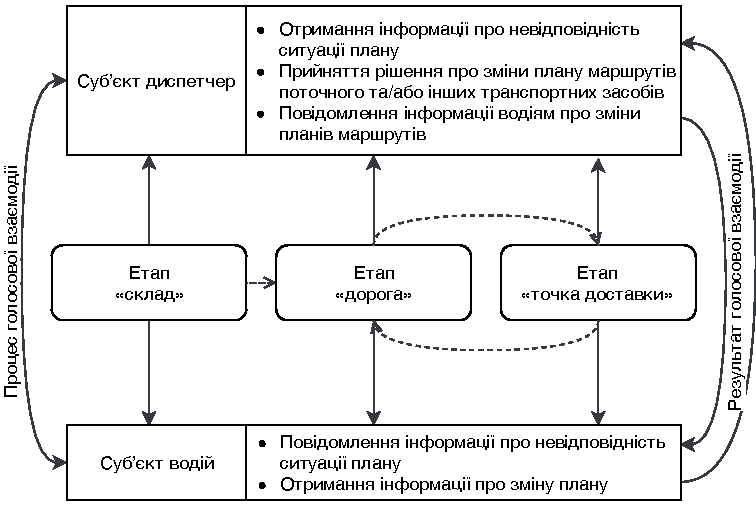
\includegraphics [width=.8\linewidth] {voice_interaction_schema}
	\caption{Модель голосової взаємодії суб’єктів дистрибуції}
	\label{img:voice_interaction_schema}
\end{figure}

Модель голосової взаємодії суб’єктів дистрибуції може бути зображена на схемі (рис. \ref{img:voice_interaction_schema}). Вона складається з трьох етапів, два останніх з яких, можуть циклічно повторюватися при наявності декількох точок доставки в маршруті. Стрілками позначено процеси голосової взаємодії, які можуть розгортатися на кожному з етапів при невідповідності плану та факту. У верхній та нижній частинах схеми показані принципові типи результатів голосової взаємодії для кожного з суб’єктів (диспетчера та водія). Ця логічна схема визначає принциповий алгоритм побудови дерева сценаріїв голосової взаємодії.


\section{Методи автоматизації руху автотранспорту в дистрибуції та параметри що впливають на сценарії голосової взаємодії} \label{sect2_2}

Транспортна логістика --- це система організації доставки, а саме переміщення будь-яких матеріальних предметів або речовин з однієї точки в іншу за оптимальним маршрутом. Транспортна логістика є частиною процесів дистрибуції, кур’єрської доставки, та інших транспортних систем, що включають в себе перевезення вантажів. Важливим етапом в процесах транспортної логістики є так званий етап «останньої милі» --- останній етап доставки вантажу з розподільчого центру до клієнта. Цей етап найменш ефективний з усього ланцюгу поставок, і може коштувати до 28\% від усієї вартості доставки. \cite{Scott_2009}

Для транспортної логістики на етапі останньої милі дуже важливим є планування маршрутів, а також моніторинг та диспетчеризація процесу доставки. Адже якісний маршрут дозволяє зменшити транспортні витрати, а моніторинг --- підвищує рівень сервісу в реакціях на позапланові ситуації. 

На жаль сьогодні в більшості компаній \todo{України} планування відбувається на достатньо примітивному рівні --- логісти визначають який транспортний засіб повезе який вантаж, але не створюють конкретний маршрут, залишаючи це рішення на водіїв. Це пов’язано в першу чергу з тим що логісти розроблюють планові маршрути вручну без залучення автоматизованих систем. Друга причина, що випливає з першої --- логісти не можуть гарантувати принципову виконуваність маршрутів, оскільки орієнтуються в більшій мірі на масо-габаритні параметри, а часові вимоги враховують лише частково. Адже масо-габаритні параметри можна порахувати сумарно незалежно від порядку об’їзду точок доставки, а часові параметри можливо перевірити лише для конкретного маршруту, побудова і прорахунок якого виходить за межі людських можливостей без використання технічних засобів. Оскільки набір точок доставки для кожного окремого транспортного засобу не є гарантовано виконуваним, то розраховувати маршрути окремих транспортних засобів не має сенсу --- потрібно вирішувати задачу в цілому для всіх точок доставки та машин, що відноситься до суттєво складнішого класу задач --- Vehicle Routing Problem (VRP).

Запровадження автоматичного розрахунку маршрутів несе в собі декілька суттєвих переваг. По перше це гарантованість принципової виконуваності маршрутів, без урахування позапланових ситуацій. По друге це підвищення рівня сервісу, адже маючи конкретний маршрут з плановим часом прибуття, ми можемо повідомити його клієнту, скоротивши його час очікування. Наприклад якщо клієнт замовив доставку з 15:00 до 18:00, він не буде 3 години \todo{<<сидіти на стільці>>} в очікуванні доставки --- він в цей час лише переважно буде знаходитися в місці доставки, але буде займатися своїми справами, можливо на щось відволічеться чи відійде на короткий час. Якщо ми повідомимо клієнту орієнтовний час доставки (наприклад з 17:00 по 17:30), то ми забезпечимо клієнту більшу свободу дій, та знизимо ймовірність того, що саме в час прибуття доставки, клієнт не зможе її прийняти вчасно, що призведе до затримки.

По трете наявність планового маршруту підвищить можливості моніторингу та реакції на позапланові ситуації. Без планового маршруту, за допомогою GPS моніторингу можливо лише побачити де перебував транспортний засіб та де він зупинявся. Але оскільки невідомий план за яким рухається водій, не зрозуміло, чи зупинка означає обслуговування точки доставки, чи водій відклав цю точку пізніше за планом і просто проїжджав повз, а зупинка --- наприклад, очікування світлофора. Крім того, не маючи плану руху транспортного засобу, не можна спрогнозувати, чи кур’єр встигає обслуговувати усі точки доставки вчасно --- можливо побачити лише факт того що якась із точок не відвідана, а замовлений клієнтом час уже вийшов. Маючи плановий маршрут, можливо в кожним момент часу спрогнозувати приблизний час прибуття на кожну з наступних точок із урахуванням можливого відставання, і побачити чи не призводить це відставання до порушення замовлених клієнтом часових вікон в майбутньому. Маючи цю інформацію набагато легше прийняти своєчасні дії --- повідомити водію про необхідність пришвидшити обслуговування точок або обговорити з клієнтом можливість перенесення часу доставки.

Варто не відкидати також і можливу економію за рахунок покращення ефективності планових маршрутів після запровадження автоматизованого планування. Тим не менше практика показує, що водій, який добре знає ввірену йому територію планує свій маршрут на достатньо високому рівні. Іноді рівень який може забезпечити водій з досвідом роботи навіть кращий за автиматизовані рішення, за рахунок наявності більш детальної інформації про карту району. Тим не менше автоматизоване планування може відв'язати якість маршрутів від людського фактору --- ріня досвіду кожного конкретного водія.

Точне вирішення задачі маршрутизації транспортних засобів неможлива для розмірів задач, з якими стикаються сучасні кур'єрські служби в містах-мегаполісах. Навіть не всі евристичні алгоритми можуть задовольнити сучасні потреби у швидкості обрахунку. В залежності від бізнес-процесів конкретної компанії та організації системи обліку та контролю за помилками, бувають ситуації коли остаточна інформація про наявні замовлення отримується лише після прибуття вантажу на розподільчий пункт і часу на планування, завантаження та відправлення кур'єрів залишається дуже мало, тому час розрахунку стандартної задачі в 2--3 тисячі точок доставки не може займати більше 30--40 хвилин.

Основна проблема впровадження систем побудови планових маршрутів на практиці полягає у спротиві інноваціям на рівні кінцевих виконавців. Водії, особливо, якщо це наймані перевізники, а не співробітники компанії, відмовляються їхати по запропонованим програмою маршрутам. Перевізників не дуже хвилює глобальна оптимальність всіх маршрутів чи рівень сервісу кінцевого клієнта, якщо до цих параметрів не прив'язана їх платня. Вони звикли отримувати маршрутний лист сформований лише за територіальними та масо-габаритними критеріями, а до часових обмежень кінцевих клієнтів ставитися доволі формально. Тому будь-які зміни звичних планів сприймаються дуже негативно, аж до саботування всього процесу. Навіть в ідеально правильному рішенні може бути необхідність заїхати на територію іншого водія для доставки в деякі точки, які інший водій не встигне виконати або необхідність доставляти точки в районі який водій погано знає, оскільки його знайомому районі в певний день мале навантаження і він може весь бути обслугований сусідами без участі цього водія, а в іншому місці навпаки навантаження велике і потрібно залучення додаткових машин. Але більшість наявних евристик орієнтуються лише на сумарну вартість, і може робити подібного роду помилки в формуванні окремого маршруту, навіть коли в цьому немає нагальної необхідності.

Таким чином постає необхідність розробки евристичного алгоритму який би максимально враховував вимоги логістів та водіїв, щодо оптимальності вибору точок з точки зору кожного конкретного маршруту, при цьому не відкидаючи глобальну оптимальність при високій швидкості обрахунку.

Практика показує, що одним з найбільш визначальних вхідних параметрів, що може сильно вплинути на результат планування та можливість його втілення у  реальність, є кількість часу, що запланована на обслуговування в точок. Адже інші параметри визначені достатньо чітко - масо-габаритні параметри відомі заздалегідь, дозволені часові вікна визначає кінцевий клієнт. Для визначення часу та відстані руху по дорозі між двома точками, є багато вже розроблених інструментів, які прогнозують результат з достатнім рівнем похибки на основі статистичних даних. Але для визначення часу обслуговування точки немає достовірного джерела інформації: ані клієнт, ані водій, ані логіст не можуть його назвати. Найбільш розповсюджена помилка --- писати всім точкам однаковий час, наприклад 10 чи 5  хвилин, незалежно від ваги та кількості вантажу який необхідно доставити або складності пошуку та під'їзду до точки доставки. Кращий варіант, який можна зустріти доволі часто - категоризація точок або конкретних замовлень, використовувати фіксований час обслуговування для всіх замовлень в категорії. Найбільш правильним варіантом, що може принести суттєву економію транспортного ресурсу при побудові планових маршрутів, є статистичний аналіз історії часу обслуговування точок. Моделювати кількість часу необхідного для виконання точки, потрібно виходячи з наступних параметрів: скільки часу використовувалося на обслуговування цієї та схожих точок в минулому, якими водіями та на яких машинах вони при цьому обслуговувалися, яку вагу, об'єм та кількість вантажу було доставлено, та інші. Питання вибору оптимального способу моделювання заслуговує окремого дослідження.

Тим не менше, для подібного статистичного аналізу, постає проблема збору цих історичних даних. Достатньо точно час зупинки можна визначити за допомогою аналізу GPS треку, але цей метод має ряд недоліків. По перше, GPS данні мають похибку, яка може збільшуватись як в залежності від якості апаратного забезпечення, так і в залежності від обслуговуваної території. Наприклад відомо що зонах висотної забудови GPS сигнал істотно погіршується, а іноді навіть втрачається повністю. Таке погіршення сигналу може згубно впливати на визначення часу зупинки або навіть факту зупинки взагалі. По друге, навіть якщо відкинути похибку GPS як несуттєву або прийнятну, постає питання співвідношення зупинок та точок доставки. У загальному випадку таке співвідношення однозначно можливе тільки якщо в заданому радіусі є лише одна зупинка та одна точка доставки. У випадках коли зупинка відбулася поза заданим радіусом, коли біля точки було декілька зупинок (в тому числі з причин хибної інтерпретації зупинки чере похибки GPS), або, як це трапляється найчастіше, одна зупинка знаходится близько до декількох точок, --- однозначно співвіднести з якої з зупинок необхідно записати час обслуговування точки неможливо. В сучасному світі, в містах мегаполісах, ситуація коли необхідно зробити декілька доставок в один багатоквартирний будинок, або сусідні будинки зі спільним двором, відбувається достатньо часто, і це автоматично унеможливлює збір та аналіз великої частини статистичної інформації про час обслуговування точки на основі GPS даних.

Отже необхідно доповнити дані GPS додатковою інформацією про те, коли водій-експедитор закінчив виконання однієї з точок в межах єдиної зупинки і почав виконання наступної точки. Практика показує що спроби зобов'язати водія в цей момент діставати телефон/планшет і вибирати відповідну команду в мобільному додатку експедитора, у кращому випадку призводить лише до того, що водій відмітить всі точки як виконані ще до або вже після виконання всіх доставок на зупинці, адже маніпуляції з планшетом потребують часу, а руки в цей момент зазвичай зайняті. Для вирішення цієї проблеми потрібен зручний для водія/експедитора інтерфейс, який би не відволікав його від основного завдання. Таким може виступати голосовий інтерфейс, який буде сприймати команди про початок та завершення виконання доставки.


\section{Методи представлення дерева сценаріїв взаємодії з урахуванням неголосової інформації} \label{sect2_3}

Для представлення дерева сценаріїв найкраще підходить орієнтовний граф, в якому вершини позначають стан системи та діалогові фрази які буде озвучувати система, а ребра --- репліки (стимулів) які можуть бути сприйняті системою в кожній конкретній вершині. Реакція на стимул може привести до переходу між станами, отже орієнтоване ребро проводиться від тієї вершини в якій стимул може буди сприйнятий, до тієї, в який стан система перейде в якості реакції на стимул. Отже множина всіх ребер, що виходять з вершини, позначають перелік стимулів, між якими треба проводити розпізнання для стану, що відповідає цей вершині.

Назва «дерево» сценаріїв використовується як сталий вираз, але реально представити всю необхідну інформацію у вигляді дерева неможливо, адже переходи між станами неминуче приводять до утворення циклів, а отже граф для представлення такої інформації підходить краще.

Нажаль такій схемі недостатньо повноти для представлення всіх можливих варіантів перебігу подій. По перше реакції системи не обмежуються переключенням станів (контекстів) що позначають доступний перелік стимулів та відтворенням діалогових фраз. Основне корисне навантаження системи --- комунікація між водієм і диспетчером та керування процесом доставки, а отже нам необхідний спосіб представлення інших реакцій на стимули, таких як відправлення певної інформації в диспетчерський центр, отримання інструкцій з диспетчерського центру, переключення внутрішніх змінних для можливості повідомити водію контекстно-залежну інформацію про "поточну" точку доставки, тощо.

По друге стимули які можуть викликати певні реакції системи і відповідно переходи між станами не обмежуються голосовими репліками сказаними водієм. Це можуть бути певні події які надійшли з інших джерел інформації, наприклад, команда від диспетчера на зміну маршруту, відміну чи перенос точки доставки, або інформація з внутрішніх джерел данних --- датчиків GPS, роботи двигуна чи відкриття дверей. Використовуючи інформацію з внутрішніх датчиків, можливо автоматизувати перехід між деякими станами, що підвищить зручність користування системою да ще зменшить кількість необхідних альтернатив для розпізнавання голосових стимулів. 

Отже для повноцінного опису ми маємо такі сутності:

\begin{itemize}
	\item \textbf{Контекст} або \textbf{Стан}, що задає перелік дозволених стимулів, які може сприйняти система в знаходячись в цьому контексті
	\item \textbf{Стимул} або \textbf{Подія} --- певна зовнішня інформація що породжує відповідну реакцію. Стимул може бути голосовою реплікою від водія, командою отриманою від диспетчера або подією породженою інформацією з внутішних датчиків, якщо вони доступні
	\item \textbf{Рекація} системи відповідно до стимулу. Рекцією може бути переключення контексту, відтворення діалогового голосового повідомлення, відправлення певної моніторингової інформації до диспетчерського центру,  переключення внутрішних змінних, тощо. Один стимул може породжувати декілька реакцій різних типів.
\end{itemize}


\section{Принципи побудови рефлекторної системи голосової взаємодії} \label{sect2_4}

\subsection{Застосування теорії несилової взаємодії як основи інтелектуальних рефлекторних систем} \label{subsect2_4_1}

Принципи побудови рефлекторних систем лежать у теорії несилової взаємодії. У роботі \cite{Teslia_2010} представлена ймовірнісна інтерпретація руху, згідно з якої єдина швидкість з якою переміщуются обʼєкти --- швидкість світла у вакуумі, а очікувана швидкість дрейфу для будь-якого матеріально об'єкта $V$ дорівнює

\[
V=c\cdot(p-(1-p))=c\cdot(2p-1)
\]

\noindent
де $p$ --- ймовірність зсуву у напрямку руху; $c$ --- швидкість світла у вакуумі

Для руху двох об'єктів $X$ та $Y$ при заданій швидкості дрейфу об'єктів $V_x$ та $V_y$ відносно деякої точки $O$, швидкість дрейфу об'єкта $Y$ відносно об'єкта $X$ ($V_{xy}$) з формули релятивістського додавання швидкостей буде дорівнювати:

\begin{equation}
\label{eq:tnv1}
	\begin{multlined}
		V_{xy}=\frac{V_y-V_x}{1-\frac{V_x\cdot V_y}{c^2}}=\frac{c\cdot(2p_y-1)-c\cdot(2p_x-1)}{1-\frac{c\cdot(2p_y-1)\cdot c\cdot(2p_x-1)}{c^2}}= \\
		=\frac{p_y\cdot(1-p_x)-p_x\cdot(1-p_y)}{p_y\cdot(1-p_x)+p_x\cdot(1-p_y)}\cdot c,
	\end{multlined}
\end{equation}

\noindent
де $p_x$ --- ймовірність зміщення об'єкта $X$ у напрямку руху; $p_y$ --- ймовірність зміщення об'єкта $Y$ у напрямку руху.

Якщо у виразі (\ref{eq:tnv1}) перейти від швидкості до ймовірності зміщення об'єкта $Y$ відносно об'єкта $X$. Отримаємо:

\begin{equation}
\label{eq:tnv2}
p_{xy}=\frac{p_y\cdot(1-p_x)}{p_y\cdot(1-p_x)+p_x\cdot(1-p_y)},
\end{equation}

\noindent
де $p_{xy}$ --- ймовірність зміщення об'єкта $X$ відносно об'єкта $Y$ у напрямку руху.

Оскільки вирази (\ref{eq:tnv1}) та (\ref{eq:tnv2}) враховують лише ті зміщення, в яких об'єкти перебувають на протиході, автор теорії висуває гіпотизу, що б'єкти Х і Y існують відносно один одного тільки в тому випадку, якщо вони знаходяться на «протиході» --- переміщаються в різних напрямках.

Згідно з зазначеною теорією кожен обʼєкт має певну власну визначеність щодо руху в одному чи іншому напрямку. 

\[
	p=\frac{i^+}{i^+ + i^-}
\]

\noindent
де $i^+$ --- розмір області визначення напрямку зміщення об'єкта у напрямку руху; $i^-$ --- розмір області визначення напрямку зміщення об'єкта проти напряму руху.

Автор вводить величини визначеності та інформованості:

\begin{equation}
\label{eq:tnv3}
d=i^+ - i^-;
\end{equation}

\begin{equation}
\label{eq:tnv4}
i=i^+ + i^-,
\end{equation}

\noindent
де $d$ --- визначеність щодо зміщення у напряму руху; $i$ --- інформованість щодо зміщення у напряму руху.

Крім того автор доводить що для руху матеріальних обʼєктів ці велечини взаємозалежні і можуть бути вираховані з формули: 

\begin{equation}
\label{eq:tnv7}
i=\sqrt{d^2+1}.
\end{equation}

З приведених вище формул можна вивести наступні залежності \cite{Teslia_2010}:

\begin{equation}
\label{eq:tnv5}
p=0.5+\frac{d}{2i};
\end{equation}

\begin{equation}
\label{eq:tnv6}
V=\frac{dc}{i};
\end{equation}

\begin{equation}
\label{eq:tnv8}
d=\pm0.5\sqrt{\frac{p}{1-p}+\frac{1-p}{p}-2}.
\end{equation}

З інформаційно-ймовірнісної інтерпретації руху, що лежить в основі теорії несилового взаємодії \cite{Teslia_2010_2}:

1. Зрозуміло, чому швидкість світла у вакуумі скінченна і максимальна. Це завжди зміщення з ймовірністю 1, а ймовірність не перевищує 1.

2. Зрозуміло, чому швидкість світла постійна відносно будь-яких рухів. Оскільки рух зі швидкістю світла - це завжди зміщення в одному напрямку, то будь-який матеріальний об'єкт рухається відносно світла тільки тоді, коли зміщується в протилежному напрямку. Їх відносна швидкість завжди дорівнюватиме швидкості світла.

3. Зрозуміла суть (розумність) деяких фізичних залежностей (релятивістське час і маса, закон збереження імпульсу). Так, вирази для релятивістського часу і маси спрощуються:$t=t_0i$; $m=m_0i$. Імпульс матеріального об'єкта пропорційний визначеності $P=m_0dc$.

4. Слідує, що об'єкти в однакових проявах --- це один об'єкт (\ref{eq:tnv2}). У цей момент вони нероздільні, і не існують відносно один одного.

5. Показує, що для фізичних законів можна отримати вирази для оперування визначеністю. З формули релятивістського додавання швидкостей отримано вираз для операції доповнення визначеності:

\begin{equation}
\label{eq:tnv9}
d_{xy}=d_yi_x-d_xi_y.
\end{equation}

Якщо відома визначеність та додаткова визначеність, то можна визначити нову визначеність:

\begin{equation}
\label{eq:tnv10}
d_y=d_xi_{xy}+d_{xy}i_x.
\end{equation}

З інформаційної інтерпретації закону збереження імпульсу отримано вираз для складання визначеності

\begin{equation}
\label{eq:tnv11}
d_\Sigma = \sum_{j=1}^N d_j.
\end{equation}

\subsection{Використання рефлекторного методу для побудови рефлекторної системи голосової взаємодії} \label{subsect2_4_2}

Принцип побудови рефлекторнх систем будуєтся на гіпотезі, що не тільки рух матеріальних обʼєктів, а й усі системи різного рівня складності підкорююся цим законам.

Для побудови інтелектуальних рефлекторних систем припускається залежність сумісної ймовної ймовірності реакції від безумовної ймовірності реакції та часткових умовних імовірностей реакції в цій системі підкорюється фізичним законам збереження імпульсу, і можуть бути розраховані по приведеним вище формулам.

Алгоритмічної основою таких систем є рефлекторний метод обчислення адекватної реакції на сукупність різних слабоструктурованих вхідних впливів.

Схема реалізації цього методу включає етапи:

1. Розрахунок визначеності для інтелектуальної системи відносно всіх вхідних впливів і можливих реакцій.

Фізична аналогія визначеності реакцій і впливів --- це імпульс матеріальних об'єктів. У такій моделі розглядаються дві групи об'єктів --- що впливають шляхом «зіткнення» та передачі власної інформації (імпульсу) об'єктам, на які здійснюється вплив (відповідно можливим реакціям). З (\ref{eq:tnv7}) та (\ref{eq:tnv8}) отримуємо:

\[
d(A_i)=\pm0.5\sqrt{\frac{p(A_i)}{1-p(A_i)}+\frac{1-p(A_i)}{p(A_i)}-2};
\]

\[
i(A_i)=\sqrt{d^2(A_i)+1};
\]

\[
d(A_i/B_j)=\pm0.5\sqrt{\frac{p(A_i/B_j)}{1-p(A_i/B_j)}+\frac{1-p(A_i/B_j)}{p(A_i/B_j)}-2};
\]

\[
i(A_i/B_j)=\sqrt{d^2(A_i/B_j)+1},
\]

\noindent
де: $p(A_i)$ --- безумовна ймовірність вибору реакції $A_i$; $d(A_i)$ --- визначеність щодо реакції $A_i$; $i(A_i)$ --- інформованість щодо реакції $A_i$; $p(A_i/B_j)$ --- умовна ймовірність вибору реакції $A_i$ (при існуванні впливу $B_j$); $d(A_i/B_j)$ --- визначеність щодо реакції $A_i$ при умові впливу $B_j$; $i(A_i/B_j)$ --- інформованість щодо реакції $A_i$ при умові впливу $B_j$.

2. З інформаційно-ймовірнісної інтерпретації формули релятивістського додавання швидкостей (\ref{eq:tnv9}) отримано додаткову визначеність, що є у впливаючих об'єктів відносно реакцій (швидкість руху впливаючих об'єктів відносно об'єктів, на які здійснюється вплив):

\[
	\Delta d(A_i/B_j)=d(A_i/B_j)\cdot i(A_i)-d(A_i)\cdot i(A_i/B_j)
\]

\noindent
де $\Delta d(A_i/B_j)$ --- додаткова визначеність щодо реакції $A_i$ яку надає вплив $B_j$.

3. З інформаційно-ймовірнісної інтерпретації закону збереження імпульсу (\ref{eq:tnv11}) розраховано сумарний вплив на реакцію інтелектуальної системи. Аналог «удару» безлічі рухомих об'єктів (відповідних дій) в об'єкти, відповідні реакцій

\[
	d_\Sigma(A_i) = \sum_j \Delta d(A_i/B_j); \\
\]

\[
	i_\Sigma(A_i) = \sqrt{\Delta d^2(A_i/B_j)+1},
\]

\noindent
де $d_\Sigma(A_i)$ --- сумарна додаткова визначеність щодо реакції $A_i$ під впливом всіх подій $B_j$; $i_\Sigma(A_i)$ --- сумарна доповнювальна інформованість щодо реакції $A_i$ під впливом всіх подій $B_j$.

4. Обчислюється нова визначеність реакцій (аналог нової швидкості руху після отриманого під час зіткнення з впливаючими об'єктами імпульсу)

\begin{equation}
\label{eq:ifron2}
d(A_i/B)=d_\Sigma(A_i)\cdot i(A_i)+d(A_i)\cdot i_\Sigma(A_i),
\end{equation}


\[
i(A_i/B) = \sqrt{d^2(A_i/B)+1},
\]

\noindent
де $d(A_i/B)$ --- нова визначеність щодо реакції $A_i$ з урахуванням впливу всіх подій $B_j \in B$; $i(A_i/B)$ --- нова інформованість щодо реакції $A_i$ з урахуванням впливу всіх подій $B_j \in B$.

5. За необхідності з (\ref{eq:tnv5}) можна обчислити сумісну умовну ймовірність реакції $A_i$ (при існуванні всіх впливів $B_j \in B$)

\[
p(A_i/B)=0.5+\frac{d(A_i/B)}{2i(A_i/B)};
\]

\noindent
де $p(A_i/B)$ --- сумісна умовна ймовірність реакції $A_i$ (при існуванні всіх впливів $B_j \in B$).

\section*{Висновки до розділу 2}
\addcontentsline{toc}{section}{Висновки до розділу 2}